%\documentclass[10pt,a4paper]{article}
\documentclass[10pt,a4paper]{scrreprt}
\usepackage[utf8]{inputenc}
\usepackage{amsmath}
\usepackage{amsfonts}
\usepackage{amssymb}
\usepackage{graphicx}
\usepackage[left=2cm,right=2cm,top=2cm,bottom=2cm]{geometry}
\usepackage{natbib}
\usepackage{bm}

\usepackage{pythonhighlight}

% integral d
\newcommand{\myd}{\;\mathrm{d}}
% overbar
\newcommand{\overbar}[1]{\mkern 1.5mu\overline{\mkern-1.5mu#1\mkern-1.5mu}\mkern 1.5mu}

\author{Yi Hu}
\title{Homogenization for Multi Field Modelling}
\subtitle{Part II: Implementation and Numerical Examples}

\begin{document}

\chapter{Derivation and Implementation}
In this chapter modelling of composite materials in multiple fields is investigated. Our target is to achieve multi scale modelling. The current work is a Unit Cell module, which supports the calculation of fluctuation in micro scale. Next homogenization is carried out to compute the averaged strain, averaged stress and ends with the calculation of effective tangent moduli. In order to obtain an effective and generic formulation energy method is exploited. The considered materials are Neo-Hookean materials and the composites containing periodic micro structures.

Details of the problem setting and derivation are presented in the following two sections. Then some issues in implementation such as alternative way of calculation are shortly discussed. The documentation rules of the code and some points about the usage are clarified in the end of this chapter.

\section{Problem Setting}
The discussion focus on the unit cell consisting of multiple materials. This unit cell can be two dimensional or three dimensional, namely a square or a cube with edge length $1$. Each material component occupies a range of domain in the cell, which are inclusions. All the inclusions possess no intersections in the domain. Multiple fields can be taken into account, such as mechanical field, temperature field and electrical field. Material types are hyperelasticity, thermomechanical Simo-Pister material (introduced in the course Elements of Non-linear Continuum Thermodynamics) and Neo-Hookean electroactive material. The energy function of electroactive material is extracted from the literature \citep{keip_two-scale_2014}. All the materials in the current material library share the common feature, i.e. no time dependency. Plasticity and viscosity are beyond our consideration in the current work.

The material energy potential per unit volume can be summarized here.
\begin{itemize}
	\item[] \textbf{Saint Venant-Kirchhoff Material} \citep{marsden_mathematical_1994}
	\begin{equation}
	\label{eq: svk}
	\psi\left( \mathbf{E} \right) = \dfrac{\lambda}{2} \left[ \text{tr}(\mathbf{E}) \right]^{2} + \mu \text{tr} \left( \mathbf{E}^{2} \right)
	\end{equation}
	\item[] \textbf{Simo Pister Material} \citep{wriggers_coupled_1992}
	\begin{equation}
	\label{eq: sp mat}
	\psi\left( \theta, \mathbf{C} \right) = \frac{1}{2}\mu_{0} \left( I_{C}-3 \right) + \frac{1}{2} \lambda_{0} \left[ \ln \left( \det \mathbf{C} \right)^{\frac{1}{2}} \right]^{2} + \left( m_{0}\Delta \theta \mu_{0}\right) \ln (\det \mathbf{C})^{\frac{1}{2}} - \rho_{0} c_{V} \left( \theta \ln\dfrac{\theta}{\theta_{0}} - \Delta \theta \right)
	\end{equation}
	\item[] \textbf{Neo Hookean Type Electroactive Material} \citep{keip_two-scale_2014}
	\begin{equation}
	\label{eq: nhk}
	\psi\left( \mathbf{C}, \mathbf{E} \right) =  \frac{1}{2}\mu_{0} \left( \text{tr}[\mathbf{C}]-3 \right) + \dfrac{\lambda}{4} \left( J^{2}-1 \right) - \left( \dfrac{\lambda}{2} + \mu \right) \ln J - \frac{1}{2} \epsilon_{0} \left( 1+\dfrac{\chi}{J} \right) J \left[ \mathbf{C}^{-1}: (\mathbf{E} \otimes \mathbf{E}) \right]
	\end{equation}
\end{itemize}
where $\mathbf{E}$ is the Green-Lagrange tensor, while $\mathbf{C}$ right Cauchy-Green tensor. Notice that $\theta$ represents temperature in the second material law and $\mathbf{E}$ in the third material is electric field intensity other than the right Cauchy-Green tensor.

\section{Derivation}
In this section the derivation concerning about solving the Unit Cell problem as well as calculating the effective tangent moduli are presented. We first formulate the total energy of composite materials, then derive equilibrium from the obtained total energy. Solving the equilibrium will give fluctuation in the micro scale. At last calculation of effective quantities is achieved, which will be required for the macro scale problem.

Motivated by the ideas from \citep{miehe_homogenization_2016}, a compact representation of field variables are presented. We denote $\mathbf{w}$ as extended displacement, which comprises the traditional displacement in mechanical problem as well as extra virtual displacements in other fields, such as temperature $T$ for the temperature field. Accordingly the strain in traditional mechanical problem should be regarded as the extended strain tensor measure here with notation $\mathbf{F}$. The extended stress can be defined in the same manner. It should be noticed that we use a slightly different notation from the one introduced in the literature \citep{miehe_homogenization_2016} (namely without star as superscript), which is for the purpose of consistency with the implementation. Since the problem in micro scale is accounted, there are two parts in each variable, namely the averaged quantity from macro scale, $\overbar{(\cdot)}$, and the fluctuation, $\widetilde{(\cdot)}$ from micro scale, which is to be solved. This relation is stated as
\begin{equation}
\label{eq: decomp}
\mathbf{w} = \overbar{\mathbf{w}} + \widetilde{\mathbf{w}}, \ \mathbf{F} = \overbar{\mathbf{F}} + \widetilde{\mathbf{F}}.
\end{equation}

The macro and micro deformation decomposition can be viewed in the following figure,
\begin{figure}[h]
  \centering
    \label{fig: mima}
    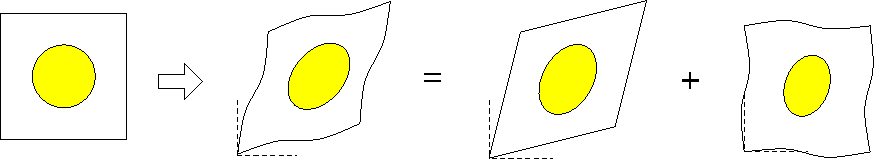
\includegraphics[width=0.8\linewidth]{../pics/mima.png}
  \caption{macro and micro deformation decomposition}
\end{figure}

One advantage of this notion is that there is then no need to treat the variable separately in the derivation. Besides the merged function feature in FEniCS can be employed and realized to its greatest extent. It is then not necessary to derive the coupled terms in stiffness matrix. All the coupled terms in stiffness matrix is calculated implicitly and automatically.

\subsection{Total Energy}
For composites total energy is the sum of energy from every component. There are two different representations of the total energy. One is used to derive equilibrium. Hence the dependency in energy is the corresponding extended displacement. The other is for the calculation of extended stress and tangent moduli. In this case the total energy should be expressed with the extended strain. Using the notation given above, these two types of total energy are stated as follows (assume there are $n$ different materials in this composite). First the original presentation of energy using extended strain is given as (here viscosity and plasticity not accounted) 
\begin{equation}
\label{eq: strain energy}
\Pi(\overbar{\mathbf{F}}, \widetilde{\mathbf{F}}) = \Pi(\mathbf{F}) = \sum^{n}_{i=1} \int \psi_{i}(\mathbf{F}) \myd{\mathbf{x}_{i}}.
\end{equation}
As extended strain is actually a function of extended displacement, meaning $\mathbf{F}=\mathbf{F}(\mathbf{w})=\mathbf{F}(\overbar{\mathbf{w}}, \widetilde{\mathbf{w}})$, the total energy can be represented as
\begin{equation}
\label{eq: disp energy}
\Pi(\overbar{\mathbf{w}}, \widetilde{\mathbf{w}}) = \Pi(\mathbf{w}) = \sum^{n}_{i=1} \int \psi_{i}(\mathbf{w}) \myd{\mathbf{x}_{i}}.
\end{equation} 

\subsection{Equilibrium}
The equilibrium of the system is built around the stationary point of total energy with respect to fluctuation,
\begin{equation}
\label{eq: equ}
\dfrac{\partial \Pi(\mathbf{w})}{\partial \widetilde{\mathbf{w}}} = \mathbf{0}.
\end{equation}
Above might be a non-linear equation. The Jacobian of this equation is therefore always needed. Denoting $\mathbf{v}$ as the test function for fluctuation, $\mathbf{w}_{\text{inc}}$ as the trial function, the weak form of (\ref{eq: equ}) and Jacobian can be expressed as
\begin{equation}
\label{eq: bi and li}
L = \dfrac{\partial \Pi(\mathbf{w})}{\partial \widetilde{\mathbf{w}}} \cdot \mathbf{v}, \ a = \dfrac{\partial L}{\partial \widetilde{\mathbf{w}}} \cdot \mathbf{w}_{\text{inc}}
\end{equation}
The whole linear equation system and stiffness matrix can be obtained through assembling. From above $L$ is the linear form and $a$ is the bilinear form. Weak formulation of (\ref{eq: equ}) is to search $\mathbf{w}_{\text{inc}}$ in $V$, such that the following holds,
\begin{equation}
a(\mathbf{w}_{\text{inc}}, \mathbf{v}) = L(\mathbf{v}),\ \forall \mathbf{v} \in \hat{V}
\end{equation}
After solving this equation fluctuation is obtained.

\subsection{Post-processing}
When it comes to post-processing, the extended strain is calculated first and the total energy of the material is expressed with (\ref{eq: strain energy}). Noticing (\ref{eq: decomp})
\begin{equation}
\mathbf{F} = \overbar{\mathbf{F}} + \widetilde{\mathbf{F}}(\widetilde{\mathbf{w}}).
\end{equation}
This can be seen as a ``mapping" of fluctuation into the strain space. The total energy is formulated with $\Pi(\mathbf{F})$ or $\Pi(\overbar{\mathbf{F}},\widetilde{\mathbf{F}})$.

The actual local extended stress is the derivative of local energy, namely
\begin{equation}
\label{eq: loc en}
\mathbf{P}_{i} = \dfrac{\partial \psi_{i}(\mathbf{F})}{\partial \mathbf{F}}.
\end{equation}
Then the averaged extended stress is the average of the above formula. When the unit cell has edge with 1, integral of $\mathbf{P}$ over the domain is the averaged quantity,
\begin{equation}
\label{eq: ave strs}
\mathbf{P}_{\text{avg}} = \sum^{n}_{i=1} \int \mathbf{P}_{i} \myd{\mathbf{x}_{i}}.
\end{equation}
This method can be implemented in FEniCS. However a more simple way of deriving is the formula,
\begin{equation}
\label{eq: ave strs 2}
\mathbf{P}_{\text{avg}} = \dfrac{\partial \Pi(\mathbf{F})}{\partial \mathbf{F}} = \dfrac{\partial}{\partial \mathbf{F}} \left( \sum^{n}_{i=1} \int \psi_{i}(\mathbf{F}) \myd{\mathbf{x}_{i}} \right).
\end{equation}
Comparing (\ref{eq: ave strs 2}) and (\ref{eq: ave strs}) the following must hold,
\begin{equation}
\label{eq: equality}
\dfrac{\partial}{\partial \mathbf{F}} \left( \sum^{n}_{i=1} \int \psi_{i}(\mathbf{F}) \myd{\mathbf{x}_{i}} \right) = \sum^{n}_{i=1} \int \dfrac{\partial \psi_{i}(\mathbf{F})}{\partial \mathbf{F}} \myd{\mathbf{x}_{i}}.
\end{equation}
For component number $n$ is independent of the extended strain $\mathbf{F}$, the sum over $n$ components could be extracted out. Then the interchange of integral and derivative needs to be shown, 
\begin{equation}
\label{eq: interchange}
\dfrac{\partial}{\partial \mathbf{F}} \left( \int \psi_{i}(\mathbf{F}) \myd{\mathbf{x}_{i}} \right) = \int \dfrac{\partial \psi_{i}(\mathbf{F})}{\partial \mathbf{F}} \myd{\mathbf{x}_{i}}.
\end{equation}
Numerical experiments show that this equality holds. Conceptually if energy depends only on the extended strain, the integral and derivative are interchangeable. More consideration should be devoted, if a valid proof is sought after. These two formulation also end with two different implementations in FEniCS.

Analogously the derivation of the averaged tangent moduli can be carried out in two different manners. 
\begin{equation}
\label{eq: tan mod}
\mathbb{C}_{\text{avg}} = \sum^{n}_{i=1} \int \mathbb{C}_{i} \myd{\mathbf{x}_{i}} = \sum^{n}_{i=1} \int \dfrac{\partial^{2} \psi_{i}(\mathbf{F})}{\partial \mathbf{F}^{2}} \myd{\mathbf{x}_{i}}.
\end{equation}
\begin{equation}
\label{eq: tan mod 2}
\mathbb{C}_{\text{avg}} = \dfrac{\partial^{2} \Pi(\mathbf{F})}{\partial \mathbf{F}^{2}} = \dfrac{\partial^{2}}{\partial \mathbf{F}^{2}} \left( \sum^{n}_{i=1} \int \psi_{i}(\mathbf{F}) \myd{\mathbf{x}_{i}} \right)
\end{equation}

Next step is to derive the homogenized parameters required for the macro scale, i.e. effective tangent moduli. This tangent moduli is the derivative of averaged extended stress $\mathbf{P}_{\text{avg}}$ with respect to macro strain $\overbar{\mathbf{F}}$. $\mathbf{P}_{\text{avg}}$ is expressed with 
\begin{equation}
\mathbf{P}_{\text{avg}} = \mathbf{P}_{\text{avg}} \left( \overbar{\mathbf{F}}, \widetilde{\mathbf{F}} \right).
\end{equation}
Hence the effective moduli is as follows,
\begin{equation}
\mathbb{C}_{\text{eff}} = \dfrac{\partial \mathbf{P}_{\text{avg}} \left( \overbar{\mathbf{F}}, \widetilde{\mathbf{F}} \right)}{\partial \overbar{\mathbf{F}}}
\end{equation}
Recalling (\ref{eq: ave strs 2}), the following formula holds, (using $\mathbf{F} = \overbar{\mathbf{F}} + \widetilde{\mathbf{F}}$ and chain rule)
\[
\mathbb{C}_{\text{eff}} = \dfrac{\partial}{\partial \overbar{\mathbf{F}}} \left( \dfrac{1}{V} \int_{\text{cell}} \mathbf{P} \myd{\mathbf{x}} \right) = \dfrac{\partial}{\partial \mathbf{F}} \left( \dfrac{1}{V} \int_{\text{cell}} \mathbf{P} \myd{\mathbf{x}} \right) : \dfrac{\partial \overbar{\mathbf{F}} + \widetilde{\mathbf{F}}}{\partial \overbar{\mathbf{F}}} =  \left( \dfrac{1}{V} \int_{\text{cell}}  \mathbb{C} \myd{\mathbf{x}} \right) : \left( \mathbb{I} + \dfrac{\partial \widetilde{\mathbf{F}}}{\partial \overbar{\mathbf{F}}} \right)
\]
\begin{equation}
\label{eq: c eff}
\xrightarrow[ V = 1]{\text{unit cell}} \mathbb{C}_{\text{eff}} = \mathbb{C}_{\text{avg}} + \int_{\text{cell}}  \mathbb{C} : \dfrac{\partial \widetilde{\mathbf{F}}}{\partial \overbar{\mathbf{F}}} \myd{\mathbf{x}} 
\end{equation}
Expressing the second term numerically is the main task in implementation, which will be discussed in the next section.

\section{Issues in Implementation}
The unit cell module is made up of three files, \texttt{cell\_geom.py}, \texttt{cell\_material.py}, \texttt{cell\_computation.py}. \texttt{cell\_material.py} defines the material in composites. Three material models are included in the material library, while user defined material can be also implemented in a easy manner. \texttt{cell\_geom.py} specifies the inclusions of the material as well as the periodic mapping in geometry. Meshes can be imported or generated within FEniCS. 3D and 2D unit cells are available. The inclusion could be circle in 2D and sphere in 3D. Rectangular inclusion and brick inclusion are also realized in the current state. Marking boundaries and corners of unit cells can work within this framework, which are often needed in the boundary conditions. The main part of this module is \texttt{cell\_computation.py}, pre-processing, formulation and solving, and post-processing are involved in this file. 

\subsection{cell\_material.py}
In this file class and functions for material definition are involved. The main part of this file is \texttt{class Material}. The definition of material starts with writing the energy function. This energy function receives invariants as the function arguments. Then one can initiate a new material with energy function and its parameters. Next define invariants and pass them into the already defined material. By calling the name of material (\texttt{\_\_call\_\_} is overrided) with the dependent functions, the instantiation of a material is complete.

Here list the definition of Saint Venant-Kirchhoff Material

\begin{python}
def st_venant_kirchhoff(E_m, nu_m):
	# Material parameters
    mu = E_m / (2 * (1 + nu_m))
    lmbda = E_m * nu_m / ((1 + nu_m) * (1 - 2 * nu_m))

	# Energy function
    def psi(inv, lmbda, mu):
        return 0.5 * lmbda * (inv[0]) ** 2 + mu * inv[1]

	# Instantiation with energy function and material parameters
    svk = Material(psi, [lmbda, mu])

    def invariant1(F):
        dim = F.geometric_dimension()
        I = Identity(dim)
        C = F.T * F
        E = 0.5 * (C - I)
        return tr(E)

    def invariant2(F):
        dim = F.geometric_dimension()
        I = Identity(dim)
        C = F.T * F
        E = 0.5 * (C - I)
        return tr(E.T * E)
	
	# Feed the invariant generators
    svk.invariant_generator_append((0,), [invariant1, invariant2])

    return svk
\end{python}

And the usage of this code is illustrated here.
\begin{python}
from dolfin import *
from cell_material import st_venant_kirchhoff

mesh = UnitSquareMesh(2, 2)
VFS = VectorFunctionSpace(mesh, 'CG', 1)
w = Function(VFS)
F = grad(w)

E_m, nu_m = 10.0, 0.3
svk = st_venant_kirchhoff(E_m, nu_m)

svk([F])
\end{python}

\subsection{cell\_geom.py}
The main class of this file is \texttt{class UnitCell}. Its instance is instantiated with a FEniCS \texttt{mesh}, and inclusions can be passed at the initiation stage or by using the member method \texttt{set\_append\_inclusion()}. Another important method is \texttt{add\_mark\_boundary()}, which will mark the boundary facets, edges or corners for later formulation of boundary conditions of problems. Inclusions are added by first instantiating an object of an inclusion class, e.g. \texttt{class InclusionCircle}. Then pass it to the instance method \texttt{set\_append\_inclusion()}. The usage is shown below,

\begin{python}
from dolfin import *
from cell_geom import UnitCell

mesh = UnitSquareMesh(40, 40, 'crossed')
inc1 = InclusionCircle(2, (0.1, 0.1), 0.5)
inc_group = {'circle_inc1': inc1}

# Direct initiation with inclusion
cell = UnitCell(mesh, inc_group)

# Set and append inclusion
cell = UnitCell(mesh)
cell.set_append_inclusion(inc_group)
\end{python}

Another focus in this file is to define periodic mapping for unit cell. It is not trivial with FEniCS, as it has its own rule of defining mapping. Two dimensional case can be referred with the example in the FEniCS forum, while three dimensional case needs more investigation of its internal mapping definition. For 2D case, mark the edges on coordinate axis as reference edges, and map other edges into these two edges. For 3D case, mark the main facets, which form between the main axis. Edges and corners not on the main axis are filtered out. The mapping then is grouped into two different categories, edge mapping and facet mapping. Edges in the same direction should be mapped to the edge on the main axis, while facet mapping is simply between two opposite facets. Detailed realization of 3D case is referred in the module. Usage of this periodic mapping is as follows,

\begin{python}
from dolfin import *
from cell_geom import PeriodicBoundary_no_corner

a, b, c = 3, 6, 9
mesh_3d = UnitCubeMesh(a, b, c)

# 3 is for 3d
FS_3d = FunctionSpace(mesh_3d, 'CG', 1, constrained_domain=PeriodicBoundary_no_corner(3))
f = Function(FS_3d)
\end{python}

\subsection{cell\_computation.py}
This is the main part of the unit cell module. Pre-processing contains merging functions and splitting functions, generate macro extended strain. Then it enters the formulation of Finite Element problem, which includes calculating total energy, imposing boundary conditions, bilinear and linear form formulation. With \texttt{comp\_fluctuation()} the fluctuation $\widetilde{\mathbf{w}}$ is obtained. Post-processing concerns about the calculation of strain, stress, averaged strain, averaged stress, averaged moduli, and effective moduli. Plotting the result with FEniCS is also wrapped for the use of material modelling.

In the pre-processing step, using \texttt{field\_merge()}, \texttt{field\_split()} or \texttt{set\_field()} makes the multi field modelling easy to handle with. Macro extended strain should also be merged and split in the case of multi field modelling. All these steps are wrapped in \texttt{input()} method.

As for the formulation and solving step, the code is rather straightforward. The boundary conditions here are Dirichlet boundary condition for fluctuation at every corner of the unit cell.

There are much more techniques in the post-processing step. The work in \ref{SchKei:2012:tho} is referred. The essential part is to derive the formula for the term 
\[
\dfrac{\partial \widetilde{\mathbf{F}}}{\partial \overbar{\mathbf{F}}}
\]
The equilibrium of the disturbed system is built with
\[
\text{div} \left[ \mathbb{C} : \left( \Delta \overbar{\mathbf{F}} + \Delta \widetilde{\mathbf{F}} \right) \right] = \mathbf{0}
\]
The weak form is given as
\begin{equation}
\label{eq: wk disturb}
\int_{\text{cell}} \delta \widetilde{\mathbf{F}} : \mathbb{C} : \left( \Delta \overbar{\mathbf{F}} + \Delta \widetilde{\mathbf{F}} \right) \myd{\mathbf{x}} = 0
\end{equation}
Then we substitute all the quantities with discretized one and rewrite the equation in matrix. Noting that $\mathbf{w}_{h}$ as the discretized fluctuation, $\mathbf{L}$ as the matrix operator that transform the extended fluctuation into its extended stress, and $\mathbf{K}$ as the stiffness matrix, then the second term in (\ref{eq: c eff}) is expressed as
\begin{equation}
\mathbf{L}^{T} \cdot \dfrac{\mathbf{w}_{h}}{\Delta \overbar{\mathbf{F}}} 
\end{equation}
The vector fraction corresponds to the derivative. This fraction is arranged in the same way as Jacobian matrix, where the $\mathbf{L}$ operator is applicable and let the dimension of the equation match with the dimension of tangent moduli matrix. The above (\ref{eq: wk disturb}) can be transformed with the matrix notation as
\begin{equation}
\mathbf{K} \cdot \mathbf{w}_{h} + \mathbf{L} \cdot \Delta \overbar{\mathbf{F}} = \mathbf{0}
\end{equation}
The overall expression of effective tangent moduli isc
\begin{equation}
\mathbf{C}_{\text{eff}} = \mathbf{C}_{\text{avg}} - \mathbf{L}^{T} \cdot \mathbf{K}^{-1} \cdot \mathbf{L}
\end{equation}

As for the implementation, the trick to obtain the corresponding matrices is to left or right multiply constant function. For averaged merged moduli, the following form is used
\begin{equation}
\mathbb{C}_{\text{avg}} = \int_{\text{cell}} \mathbf{F}_{\text{test\_const}}: \mathbb{C} : \mathbf{F}_{\text{trial\_const}} \myd{\mathbf{x}}.
\end{equation}
The corresponding code for this expression is 
\begin{python}
# Trial and test function to multiply with
F_const_trial = TrialFunction(self.strain_const_FS)
F_const_test = TestFunction(self.strain_const_FS)

# Derivate in the test and trial function direction, the same with left and right multiply
dPi_dF = derivative(self.Pi, self.F_merge, F_const_test)
ddPi_dF = derivative(dPi_dF, self.F_merge, F_const_trial)
# Integral over the unit cell
C_avg = assemble(ddPi_dF)
\end{python}

The same trick applies to the second term of the effective tangent moduli, where constant trial function is chosen for $\overbar{\mathbf{F}}$. The implementation is as follows. 
\begin{python}
# Trial function
F_bar_trial = TrialFunction(self.strain_const_FS)
# F_w is the linear form generated from the fluctuation solving step
L2 = derivative(self.F_w, self.F_bar_merge, F_bar_trial)
B2 = assemble(L2)

# Sensitivity method is just for efficient implementation of calculating K\L
LTKL2 = self.sensitivity(B2)
\end{python}

\section{Documentation}
This unit cell module contains a Python documentation in the original code. Docstrings are used in the implementation. The format of docstring is reStructuredText. A Sphinx documentation manual is generated for the module. Besides, the usage of this module is clarified with examples and the unittest cases are also included for testing the new functionalities.

\end{document}
